%\section{Introduction}
\section{Background} 
Vessel detection and trajectory prediction is a critical subfield of intelligent maritime surveillance. It focuses on the automatic identification and monitoring of
ships using satellite sensors and movement data. This supports applications including traffic management, fishery enforcement, smuggling prevention, and national
security. These are some fields where continuous and reliable vessel monitoring is
crucial. Recent deep trajectory frameworks have improved  this domain by leveraging physics-guided diffusion models to accurately reconstruct long-term missing trajectories~\cite{10.1145/3637528.3672086}, while tracking layouts utilize spectral clustering with bidirectional LSTM cells~\cite{jmse9091037} or deep probabilistic networks~\cite{s22052058} to forecast vessel paths. Early maritime vessel detection relied on classical signal processing methods
and shallow machine learning techniques. Comprehensive systematic surveys explain that while traditional C-band frameworks formed early baselines,they were struggling to optimize target boundaries across varying pixel configurations~\cite{10620443, jmse9121408}. Optical methods relied on manually extracted features including texture, shape and color from image regions, which were
then used by machine learning classifiers to identify the vessels. On the other hand,
SAR-based methods depended on radar signal pattern analysis. In this approach,
changing sea conditions often caused high false detections, reducing real-world operation reliability. \\


The emergence of deep convolutional neural networks introduced a significant advancement in vessel detection. Region-based CNNs established deep learning as the
dominant approach for vessel detection. For instance, context-aware region-based CNN architectures utilized multilayer feature fusion and achieved superior localization scores across extensive baseline counts of 7,986 fully labeled vessels~\cite{rs9080860}. This led to the development of two-stage
and one-stage architectures that automatically learned robust features from data
without relying on manually extracted features. Single-stage models such as optimized YOLOv5s frameworks demonstrate this capability, securing an Average Precision of 95.36\% in offshore settings and 92.27\% across complex inshore regions~\cite{10.3389/fmars.2022.1086140}. This significantly improved adaptability to complex maritime environments. SAR-based vessel detection adopted the similar transition, enabling precise target localisation through advanced spatial feature extraction. Earlier methods struggled with various vessel sizes and crowded port environments. Additionally, environmental factors such as sea conditions, lighting, and weather often reduced detection reliability. \\


Although vessel detection has advanced significantly with deep learning, effective maritime surveillance also depends on vessel movements tracking over time. Maritime surveillance has traditionally depended on the Automatic Identification System (AIS) as the primary source of vessel position and kinematic data. AIS provides timestamped reports of latitude, longitude, SOG, and COG, which form the foundation of most trajectory analysis frameworks. However, AIS is a self-reporting protocol whose effectiveness depends on vessel cooperation. Signal gaps can occur because of technical failures and coverage limitations or even be created by intentional deactivation, particularly during illegal maritime activities. These gaps can reduce the reliability of cooperative surveillance systems. \\

Despite its widespread adoption, AIS suffers from substantial data quality issues in practice. Studies on large-scale AIS datasets have shown that trajectory gaps of several hours are common, with some vessel paths missing up to 60\% of expected position reports during long ocean transits~\cite{10.1145/3637528.3672086}. In coastal and port-dense regions such as the Norwegian fjords, vessels frequently operate in overlapping radio coverage zones, causing packet collisions that degrade positional accuracy~\cite{s22052058}. Trajectory prediction experiments using Bi-LSTM on AIS data collected from Busan Port demonstrated that clustering vessel routes by behavioral similarity prior to modeling reduced prediction error by a significant margin compared to training on raw unsegmented trajectories~\cite{jmse9091037}. Furthermore, fusion studies combining SAR imagery with AIS self-reports revealed systematic discrepancies between declared and observed vessel positions, particularly in high-traffic separation schemes where positional offsets of several hundred metres were recorded~\cite{7093130}. More recently, physics-guided diffusion models evaluated on the Danish AIS benchmark achieved state-of-the-art trajectory imputation performance, reducing displacement error by over 30\% relative to LSTM-based baselines on gaps exceeding three hours~\cite{10.1145/3637528.3672086}. Knowledge graph-enhanced imputation methods have further demonstrated that incorporating maritime domain rules such as COLREGS constraints into the reasoning process yields trajectories that are not only more accurate but also more interpretable and regulation-compliant~\cite{liu2026vista}. \\

These limitations led to more advanced and context-aware approaches. Vessel detection evolved to use attention mechanisms and multi-scale feature learning, while trajectory analysis adopted physics-informed diffusion models and knowledge graph-based frameworks, improving explainability and supporting missing trajectory reconstruction. Most current methods are now evaluated using large AIS datasets. However, challenges still remain in detecting small vessels in cluttered environments and reconstructing trajectories of dark vessels. \\



\section{Rational of the Study or Motivation}
The inability to effectively monitor sea activities may lead to numerous issues, such as illegal trade, unauthorized vessels entering, trespassing, and putting many human lives in danger. Additionally, monitoring a vessel using AIS data becomes challenging due to issues like reduced network strength, signal attenuation, spoofing, and especially when transponders are intentionally turned off, making it significantly harder to track a vessel in its normal state. For these reasons, maritime monitoring relies heavily on SAR and optical imagery. Each of these has its specific limitations; SAR struggles with noise speckling and grainy images, while optical systems are hampered by adverse weather, remote oceans, and nighttime conditions. Due to these problems, unlawful ships frequently exploit the situation. A significant issue in current detection is the absence of a system capable of integrating data from scattered sensors, monitoring silent ships, and making predictions; this also poses a considerable risk for high-seas piracy and environmental infractions related to transnational smuggling. Recent studies confirmed that AIS data may face disruption  for more than 6 hours caused by signal manipulation and system failures worsening maritime surveillance system~\cite{10.1145/3637528.3672086}. This motivates the creation of an intelligent sensor capable of detecting ghost ships while predicting paths in challenging conditions, utilizing physics principles, oceanographic knowledge, and maritime regulations.\\

\section{Problem Statement}
The identification of ships at sea and route detection remains a significant challenge with existing systems. Currently, AIS data significantly contributes to determining ship positions and tracking their trajectories, providing time-stamped geographic coordinates, speed over ground (SOG), and course over ground (COG) information. Conversely, it greatly relies on ocean regions or vessel equipment, as any failure can cause the AIS to malfunction, resulting in a total lack of visibility for the existing monitoring system. Moreover, it could be effortlessly turned off, resulting in numerous problems such as illegal trade, unpermitted ships entering, trespassing, and endangering many lives. More than 20\% of global catch is estimated to be from Illegal, Unreported, and Unregulated (IUU) fishing, and the biggest IUU offenders are fleets that do not use AIS~\cite{paolo2022xview3}. In addition to the reliance on a single modality, vessels can easily become obscured because of poor weather conditions for optical images and grainy images for SAR due to high ocean waves. Present multi-model systems often operate ineffectively as they lack filters for selecting the appropriate image when circumstances vary. Similarly, current systems generate path predictions by treating vessels as distinct kinematic entities and do not account for oceanic physics or international maritime regulations (COLREGS). \\

Consequently, it is crucial to develop a model-model system that can operate independently of AIS data and identify both visible vessels and “ghost ships,” as well as perform trajectory prediction, by synthesizing fragmented information from various sensors and considering marine regulations for path prediction and vessel identification. 




\section{Objective}
The principal focus of this research is to build a trustworthy and effective multimodal deep learning system aimed at improved vessel detection and motion prediction amid adverse maritime surveillance conditions. The proposed framework fuses SAR imagery along with optical imagery via physics driven probabilistic modelling acting as the core of the system architecture. In order to accomplish the goal, this research seeks to:

\begin{enumerate}
    \item Develop a strongly fused SAR-Optical pipeline which combines the complementary features of individual senses for precise vessel detection.
    
    \item Construct an independent positional evidence leveraging SAR-Optical imagery that facilitates the identification of AIS-non-compliant vessels and AIS-dark vessels in order to mitigate dependence on AIS reports.
    
    \item Integrate multi-scale feature extraction with adaptive attention mechanisms to improve detection of small vessels under challenging sea-state and clutter conditions.
    
    \item Design a physics-guided trajectory prediction model that incorporates the vessel's kinematic constraints to produce physically realistic vessel path reconstructions.

     \item Ensure temporal consistency and predicted trajectory explainability by maintaining state estimates and incorporating COLREGS rules and vessel behavior semantics through Ship-Domain Knowledge Graph.
     
    \item Evaluate the framework against real-world maritime surveillance scenarios including dark vessel monitoring, collision risk assessment, and anomaly detection. 
\end{enumerate}


\section{Methodology in Brief }

In this research we have tried to build a multi-modal deep learning network that takes both the SAR and optical image to figure out the exact trajectory of the target ship. Firstly, upon receiving the optical image the preprocessing stage starts where the image is enhanced using contrast adjustment (CLAHE) and noise reduction techniques(Median + bilateral filter). After that, the enhanced image goes through a deep-learning based detection network which consists of an ELAN-ODConv backbone, an ASFFPredict-BiFPN multiscale feature fusion neck, and an ELANH-SPDC detection head.The backbone learns discriminative ship representations, while the multiscale fusion module combines information from different features so that it can improve the robustness of different sizes of ships. And lastly, the ‘Rotation Head’ prediction module estimates the  bounding box of the target ship. Figure~\ref{fig:methodology} shows the whole process in brief. \\
\begin{figure}[htbp]
    \centering
    % \includegraphics[width=\textwidth]{images/diagram.png}
    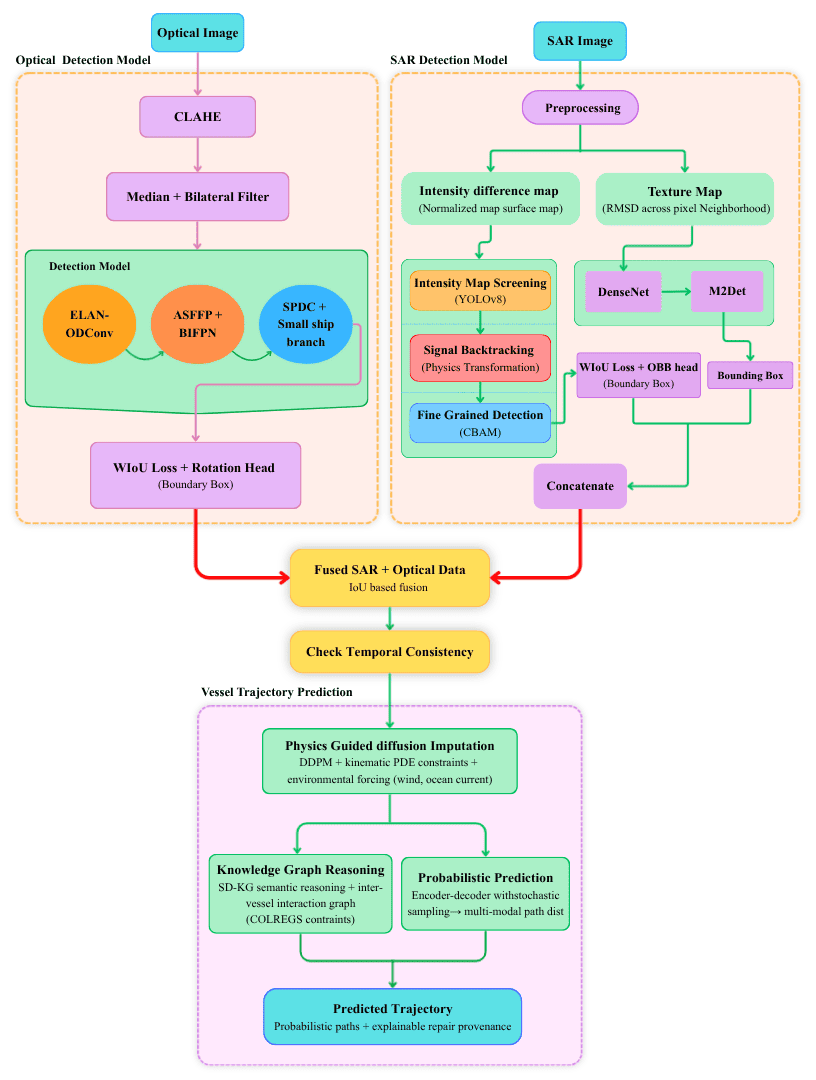
\includegraphics[width=\textwidth]{images/diagram_vertical.png}
    \caption{Methodology in Brief}
    \label{fig:methodology}
\end{figure} 


On the other side of the model ,when the SAR image is received, the model starts  normalizing decibel levels and removing speckles , to lessen the important effect of sea clutter. This approach segments the procedure into an Adaptive Dual-Path Feature Separation for Different SAR Signatures by concurrently producing  intensity map alongside a texture map, utilizing a Root Mean Square Deviation evaluation among adjacent pixels to differentiate minor vessels from bigger ships. Subsequently, a designated threshold on a YOLOv8 analyzes the intensity maps to detect micro-scale marine vessels in turbid zones and highlights unclear areas to activate a signal backtrack. This backtracking approach undoes the image generation procedure to extract unprocessed complicated signals.The model then observes the satellite's hypotenuse measurement to complete a physics-constrained path gap filling of the vessel's trajectory, prior to inputting the synchronized data routes into a feature-rich network combined with M2Det's multi-scale forecasting.This multi-modal incorporation employs confidence-aware sensor fusion among models via CBAM attention, WIoU Loss, and an OBB prediction head, which gives an accurately oriented bounding box of the target ship and its confidence score.\\

After we get the bounding boxes from both the models,the fusion takes place where it combines ship detections from SAR and optical imagery by first comparing their bounding boxes and calculating IoU (Intersection over Union) value  to measure the overlap between the two boxes. Boxes that have a higher IoU value are merged together indicating that they have captured the same ship and boxes below the threshold are kept separate as different vessels. For merged boxes, the final fused bounding box is created by averaging their confidence scores, center coordinates (x, y), and dimensions (w, h). Then, the fused picture  goes through the temporal consistency check where the system goes through multiple frames at once and for each detected ship, the Euclidean distance is calculated between the centroids of bounding boxes to figure out if the same ship had its presence over the multiple frames.\\

Lastly using these combined coordinates, the trajectory reconstruction component focuses on creating the ship’s trajectories when AIS signals are missing or intentionally disabled by dark ships. The large gaps between known positions are imputed using a physics-guided diffusion model (DDPM). The model is conditioned on kinematic constraints and environmental forcing such as wind and ocean currents to ensure physically consistent interpolation. The imputed trajectory is then processed through two parallel branches. One branch utilizes a ship-domain knowledge graph (SD-KG) for context-aware reasoning and explainability based on historical vessel behavior and COLREGS rules. The other branch leverages an encoder-decoder that generates multiple possible paths to capture motion uncertainty. Outputs from both branches are fused to generate the final reconstructed trajectory. 
 \\





\section{Scopes and Challenges}
This research aims to develop a multimodal deep learning framework that detects maritime vessels and predicts their trajectories using SAR and optical satellite imagery.  It covers diverse maritime environments such as open-sea, inshore, and port environments under varying weather and lighting conditions, with a specific focus on detecting small vessels under 20 meters and reconstructing AIS-dark vessel trajectories. It also emphasizes maintaining temporal consistency across AIS gaps and signal disruptions. The trajectory component addresses missing vessel positions imputation using physics-guided diffusion modeling conditioned on kinematic constraints. Context-aware prediction is achieved through COLREGS rules and vessel behavioral semantics.\\

In order to implement this framework several key challenges must be addressed. In the detection domain, SAR imagery is often degraded by speckle noise and strong sea clutter that obscure small or concealed vessel signatures. Meanwhile, optical imagery struggles under adverse weather, cloud cover, and nighttime conditions, which are often exploited by illicit vessels. Intelligently fusing both modalities remains a key challenge, as each sensor’s reliability significantly varies depending on environmental conditions. In the trajectory domain, AIS gaps caused by satellite coverage limitations, technical failures, and deliberate deactivation disrupt continuity of vessel movement histories. Reconstructing missing segments while respecting real ocean physics and COLREGS rules is beyond what conventional interpolation or independent kinematic models can achieve. Additionally, ensuring that the framework generalizes across diverse vessel types, geographic regions, varying sea conditions, and unseen dark vessel behaviors — without overfitting to a specific dataset or operational condition — remains a major unsolved research challenge.






